%%%%%%%%%%%%%%%%%%%%%%%%%%%%%%%%%%%%%%%%%%%%%%%%%%%%%%%%%%%%%%%%%%%%%%%%%%%%%
%%%                              LISTPLOT                                 %%%
%%%%%%%%%%%%%%%%%%%%%%%%%%%%%%%%%%%%%%%%%%%%%%%%%%%%%%%%%%%%%%%%%%%%%%%%%%%%%
\newpage
\subsubsection{Listplot}
List plots can be used to display line curves with up to 8 differently scaled
axes in a common plot window.
\label{sec:uilistplot}
\index{Plot!Listplot}

\input{diagrams/ui_listplot_list}
\index{LISTPLOT@\LISTPLOT}
\input{diagrams/ui_listplot_vertical_graph_list}
\input{diagrams/ui_listplot_horizontal_graph_list}
\input{diagrams/ui_listplot_option_list}

\index{CAPTION@\CAPTION!listplot option}
\index{SIZE@\SIZE!listplot option}
\begin{tabularx}{\textwidth}{l|X}
options       & description \\ \hline
\verb+string+ & defines the label string for the print menu button.\\
\CAPTION      & defines the caption text that will be printed in the right most
                column of the plot. The identifier must be a previously declared stream.
                (see section \nameref{sec:streamer} on page \pageref{sec:streamer})\\
\SIZE         & x, y in pixel \\
\end{tabularx}

\input{diagrams/ui_listplot_horizontal_graph_item}
\input{diagrams/ui_listplot_graph_option}

\index{XAXIS@\XAXIS!ui\_manager listplot}
\index{AXES\_ORIGIN@\AXESORIGIN!ui\_manager listplot}
\index{LOG\_X@\LOGX!ui\_manager listplot}
\index{LOG\_Y@\LOGY!ui\_manager listplot}
\index{SAME\_YRANGE@\SAMEYRANGE!ui\_manager listplot}
\begin{tabularx}{\textwidth}{l|X}
graph options        & description \\ 
\hline
{\verb+string+}     & defines the graph title.\\
{\verb+identifier+} & defines the graph title that will be printed at the top 
                       of the plot. The identifier must be a previously declared stream.
                       (see section \nameref{sec:streamer} on page \pageref{sec:streamer})\\
\XAXIS               & defines the data item whose values give the x-coordinates\\
\AXESORIGIN          & defines the origin for all y-values\\
\LOGX                & the x-axis is scaled logarithmically\\
\LOGY                & the y-axis is scaled logarithmically\\
\SAMEYRANGE          & sets all y-axes to the the same range\\
\LABEL               & TODO \\
\end{tabularx}

\input{diagrams/ui_listplot_item}
\index{Scale factors!listplot item}
\begin{tabularx}{\textwidth}{l|X}
plot item         & description \\
\hline
\verb+identifier+ & references the data to be plotted (data item, stream-id). \\
\verb+scale+      & a scale factor (see section \nameref{sec:scale} page \pageref{sec:scale}). \\
\end{tabularx}

\input{diagrams/ui_listplot_item_option}

\index{LINESTYLE@\LINESTYLE!listplot option}
\index{LINEAR@\LINEAR!listplot option}
\index{STEP@\STEP!listplot option}
\index{DISCRETE@\DISCRETE!listplot option}
\index{LABEL@\LABEL!listplot option}
\index{UNIT@\UNIT!listplot option}
\begin{tabularx}{\textwidth}{l|X}
plot item options & description \\
\hline
\verb+string+    & defines the unit string.\\
\verb+identifier+ & streamer-identifier.\\
\LINESTYLE        & defines the line style \\
\LINEAR           & the points are connected by straight lines\\
\STEP             & the points are connected with horizontal and vertical lines\\
\DISCRETE         & the points are not connected.\\
\LABEL            & string or stream identifier \\
\UNIT             & string or stream identifier \\
\end{tabularx}

\newpage
The following example shows the configuration of a 2D-plot 
and how it will
be displayed by \INTENS{} (see page \pageref{fig:listplot})


\begin{boxedminipage}[t]{\linewidth}
\begin{alltt}
  \LISTPLOT  
    curve_plot\{ "Plot" \} ( 
       ( magn_curve \{"Magnetizing curve", \XAXIS=iMag\}
         ( psiMag\{"[Vs]"\} ), 
         x_i2  \{"Rotor current", \XAXIS=speed*60\{"1/min"\} \} 
         (i2\{"[A]"\} ) 
       ),
       ( x_torque\{"Induction Motor", \XAXIS=speed*60\{"1/min"\} \}
         ( torque*1e-3\{"[kNm]"\}, i1\{"[A]"\}, cos )
       )
    );
  \FORM
    curve_form (
       ( curve_plot )
    );
\end{alltt}
\end{boxedminipage}

\vspace{1cm}

\begin{figure}[h]
   \begin{center}
      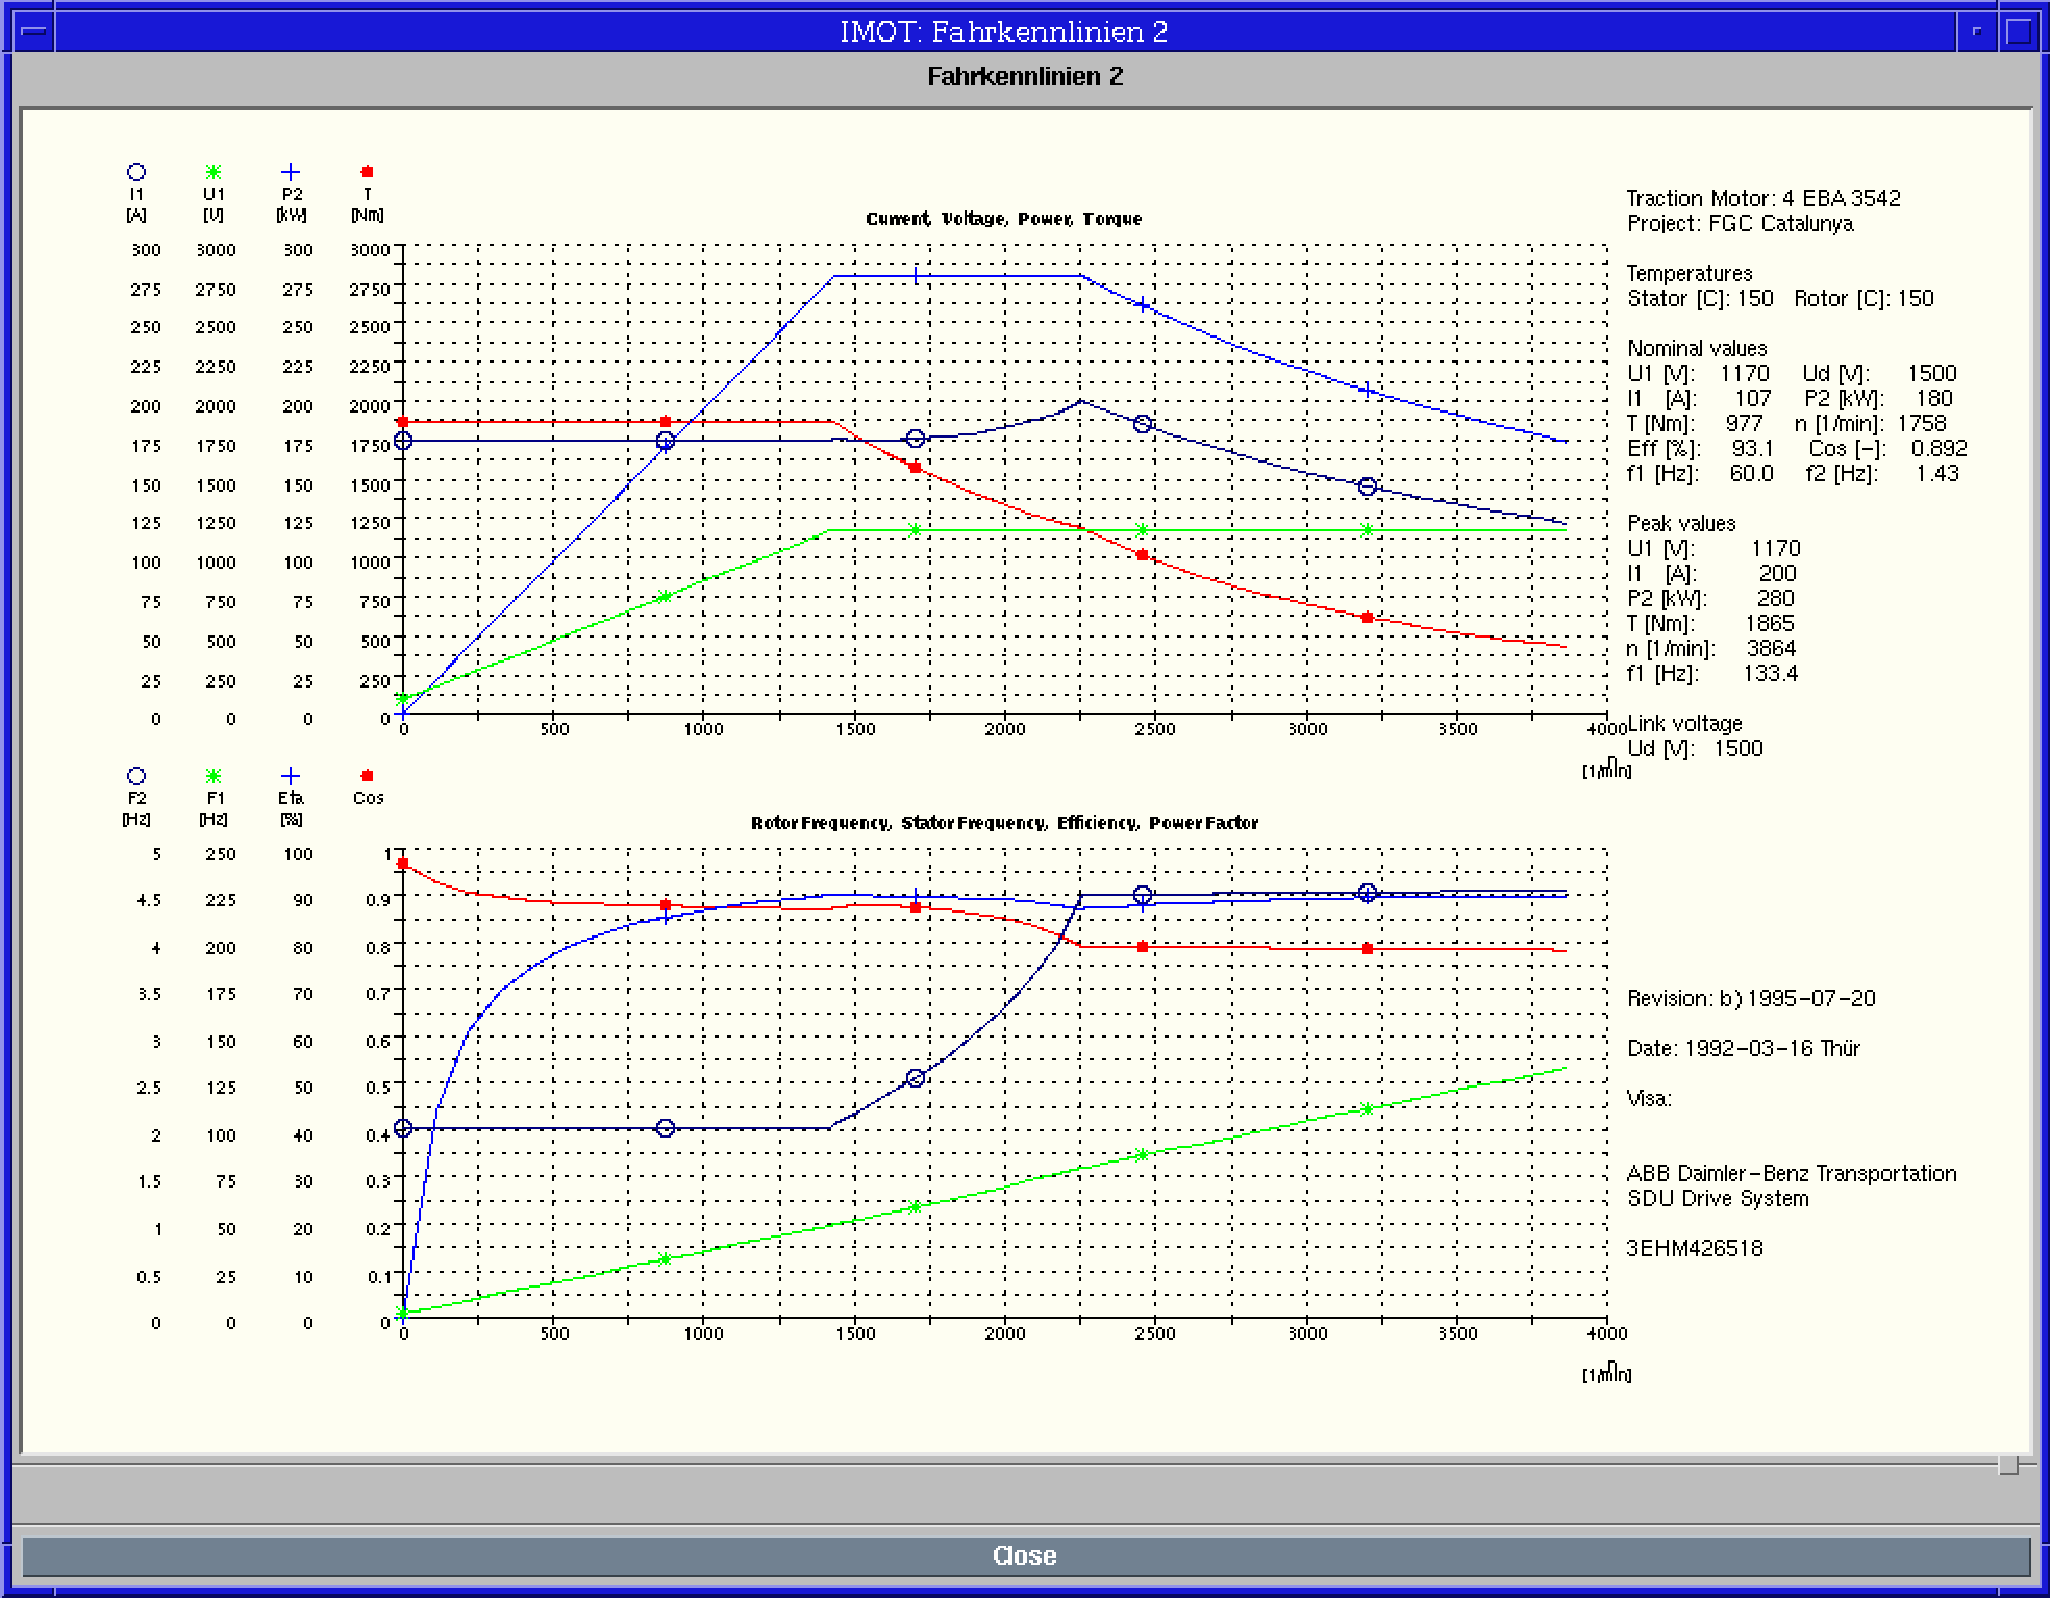
\includegraphics[width=\linewidth]{grab_listplot}
      \caption{\LISTPLOT{} diagram with 2 plots}
      \label{fig:listplot}
   \end{center}
\end{figure}
